% TeX eps-loader file generated by PlotPosteriorDistributions.m (Dynare).
% 01-Oct-2019 22:16:09
 
\begin{figure}[H]
\psfrag{RA}[1][][0.5][0]{$ {r_{A}} $}
\psfrag{PA}[1][][0.5][0]{$ {\pi^{(A)}} $}
\psfrag{GAMQ}[1][][0.5][0]{$ {\gamma^{(Q)}} $}
\psfrag{TAU}[1][][0.5][0]{$ {\tau} $}
\psfrag{NU}[1][][0.5][0]{$ {\nu} $}
\psfrag{PSIP}[1][][0.5][0]{$ {\psi_\pi} $}
\psfrag{PSIY}[1][][0.5][0]{$ {\psi_y} $}
\psfrag{RHOR}[1][][0.5][0]{$ {\rho_R} $}
\psfrag{RHOG}[1][][0.5][0]{$ {\rho_{g}} $}
\centering
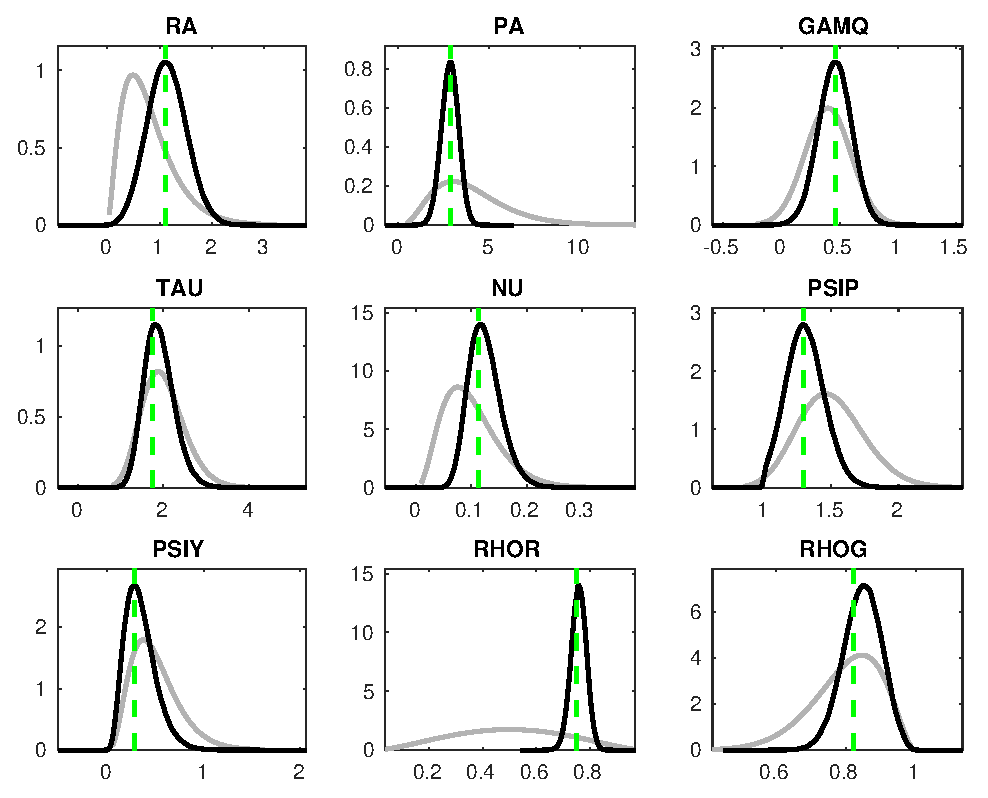
\includegraphics[width=0.80\textwidth]{AnSchoModTheBuilder/Output/AnSchoModTheBuilder_PriorsAndPosteriors1}
\caption{Priors and posteriors.}\label{Fig:PriorsAndPosteriors:1}
\end{figure}
 
\begin{figure}[H]
\psfrag{RHOZ}[1][][0.5][0]{$ {\rho_z} $}
\psfrag{SIGR}[1][][0.5][0]{$ {\sigma_R} $}
\psfrag{SIGG}[1][][0.5][0]{$ {\sigma_{g}} $}
\psfrag{SIGZ}[1][][0.5][0]{$ {\sigma_z} $}
\centering
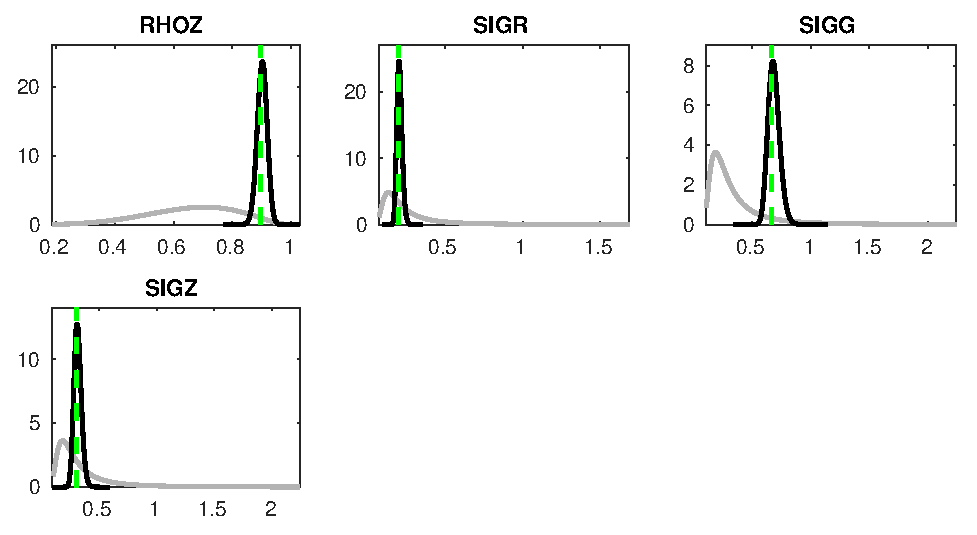
\includegraphics[width=0.80\textwidth]{AnSchoModTheBuilder/Output/AnSchoModTheBuilder_PriorsAndPosteriors2}
\caption{Priors and posteriors.}\label{Fig:PriorsAndPosteriors:2}
\end{figure}
 
% End of TeX file.
